\chapter{Design}

The system design follows the architecture from \cref{fig:sys:arch} where many
classes uses names that easily can be mapped to what they correspond to in the
architecture. The class diagram can be seen in \cref{fig:design:class}.

\begin{figure}[H]
    \centering
    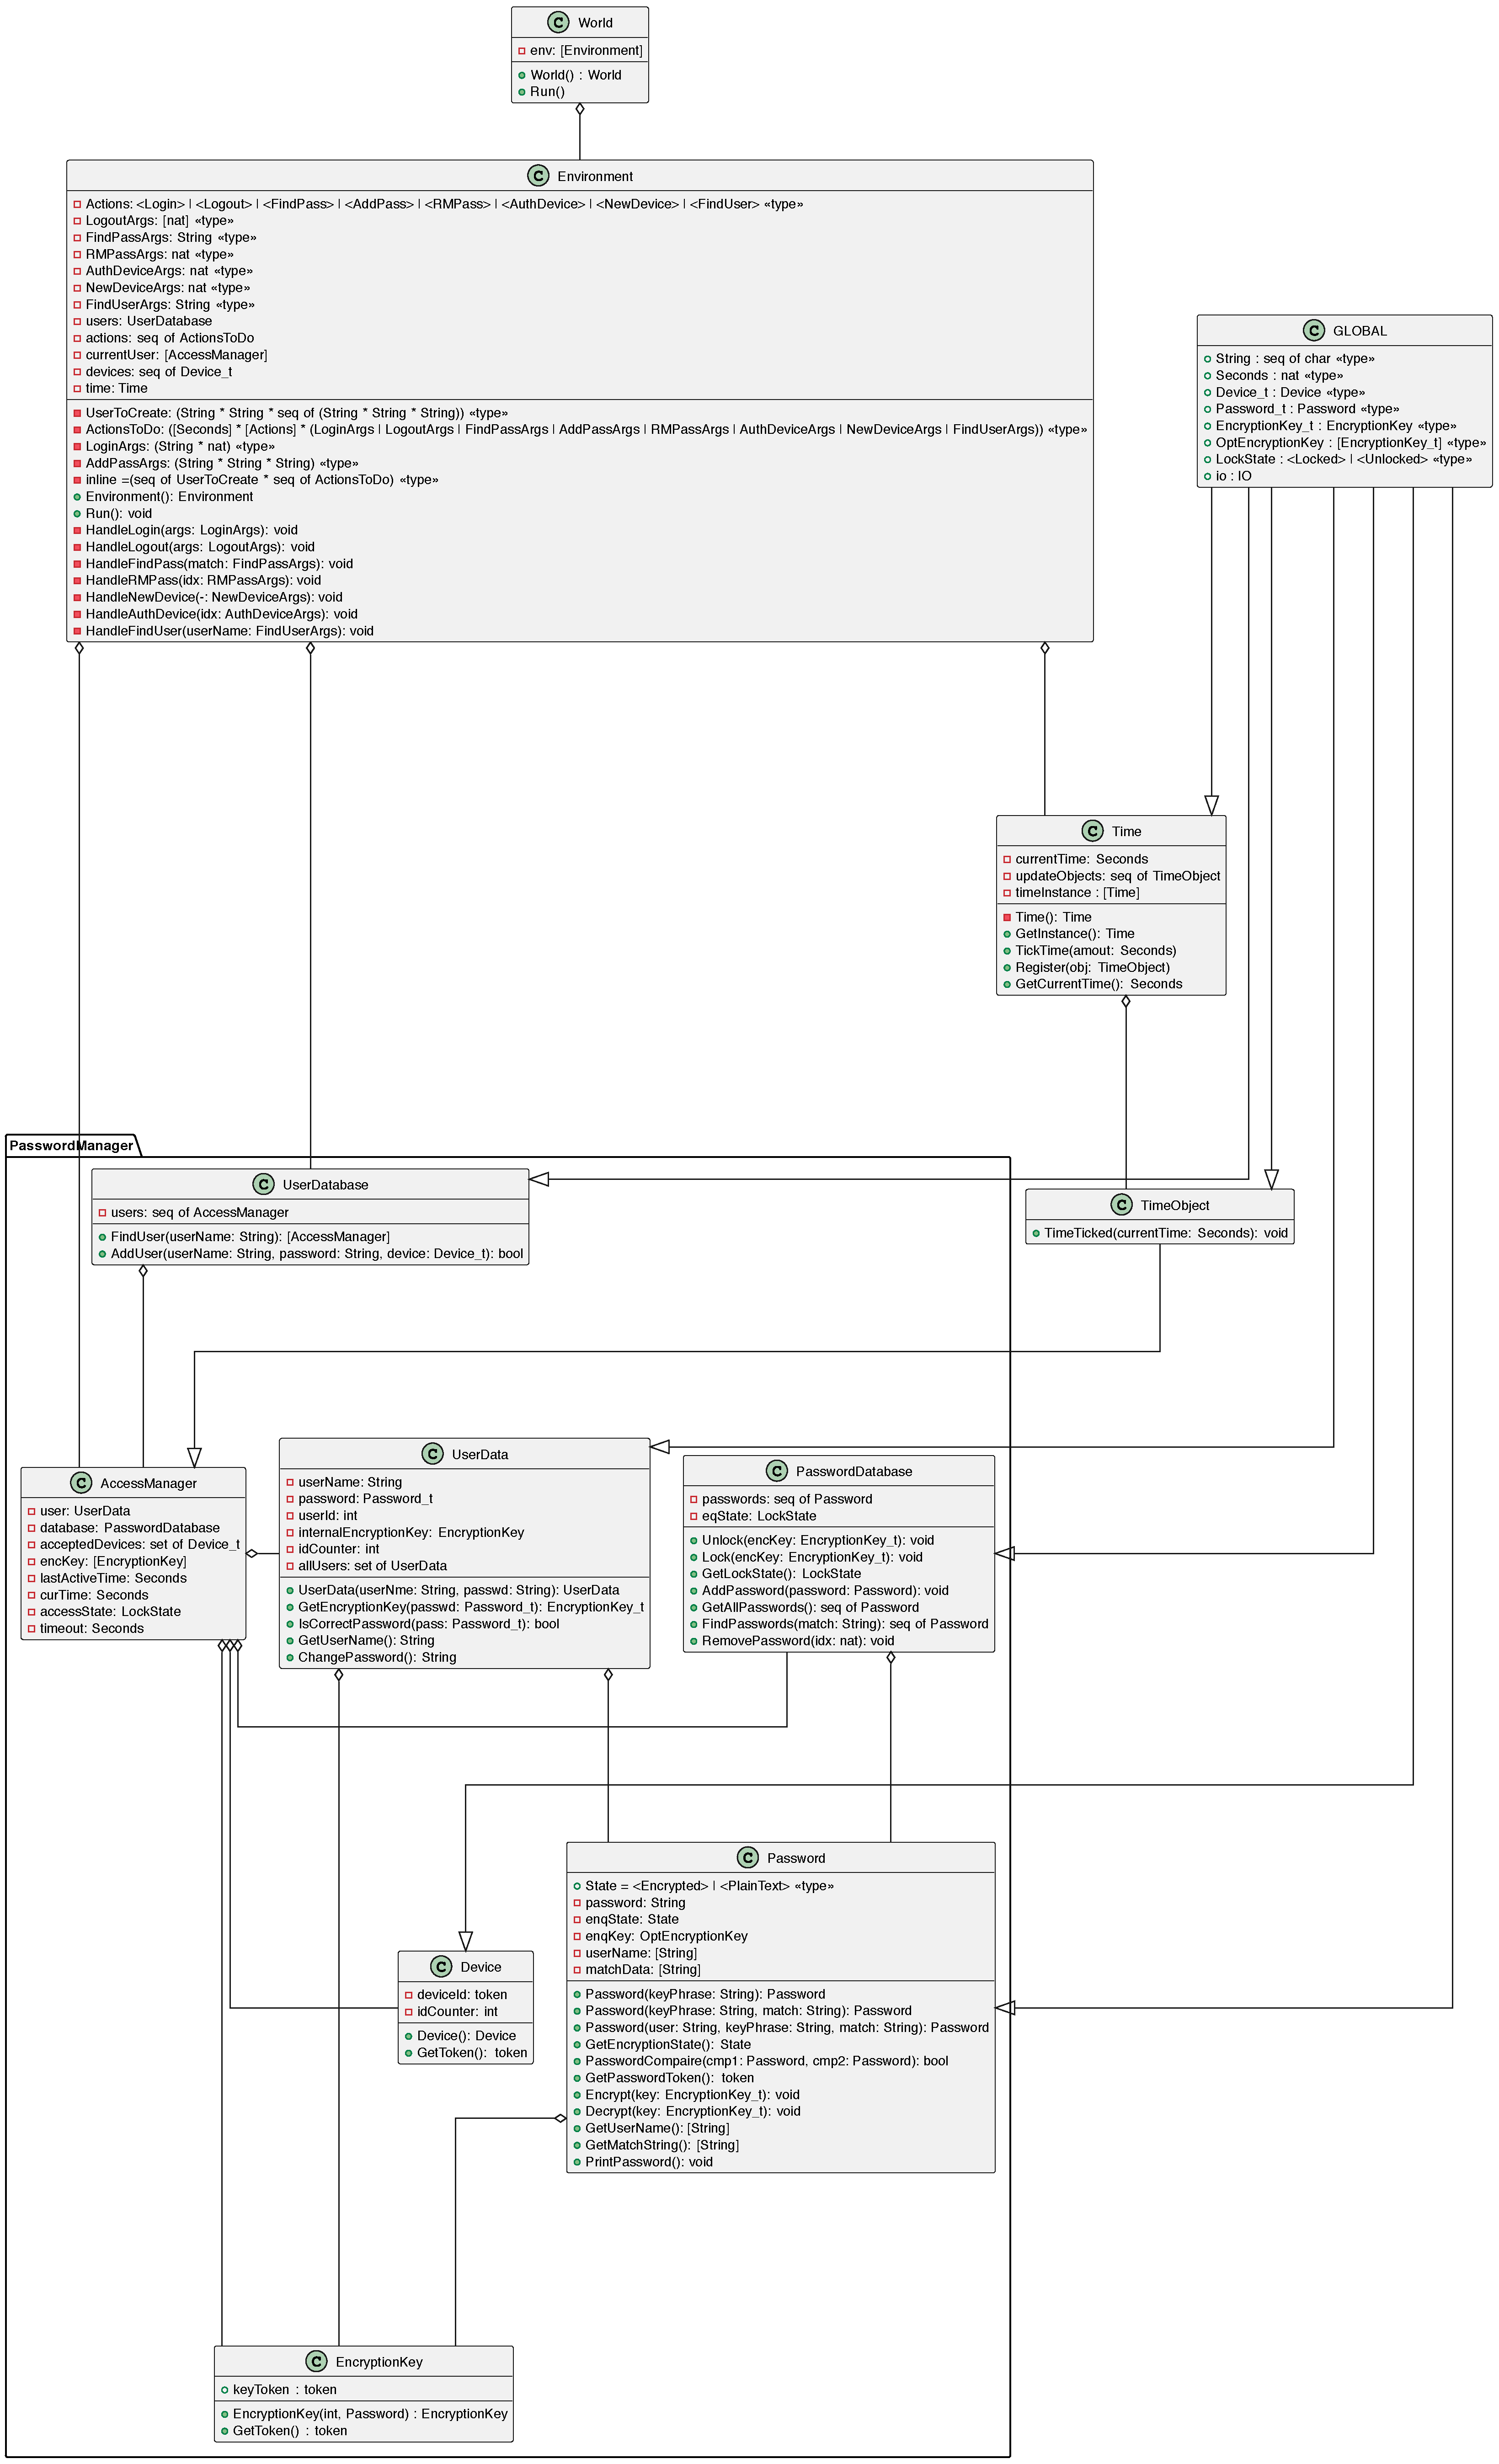
\includegraphics[width=13cm]{prj/figs/ClassDiagram.pdf}
    \caption{Class diagram for the Password Manager. Unit test classes are omitted.}
    \label{fig:design:class}
\end{figure}

The design is largely following the sequential design model. However since the
Time is implemented as a singleton and is not used by the world, there is no
reason for it to initialize it, when it is the environment that ends up using
it in the scenario. Due to the model also to be able to react on different time
events, a time object is also implemented, so classes can handle each time tick
when needed.

Unit testing this is automated with the combinatorial testing functionalities
that VDM++ have. An simplified class diagram of how the unit testing is done is
shown in \cref{fig:design:test}

\begin{figure}[H]
    \centering
    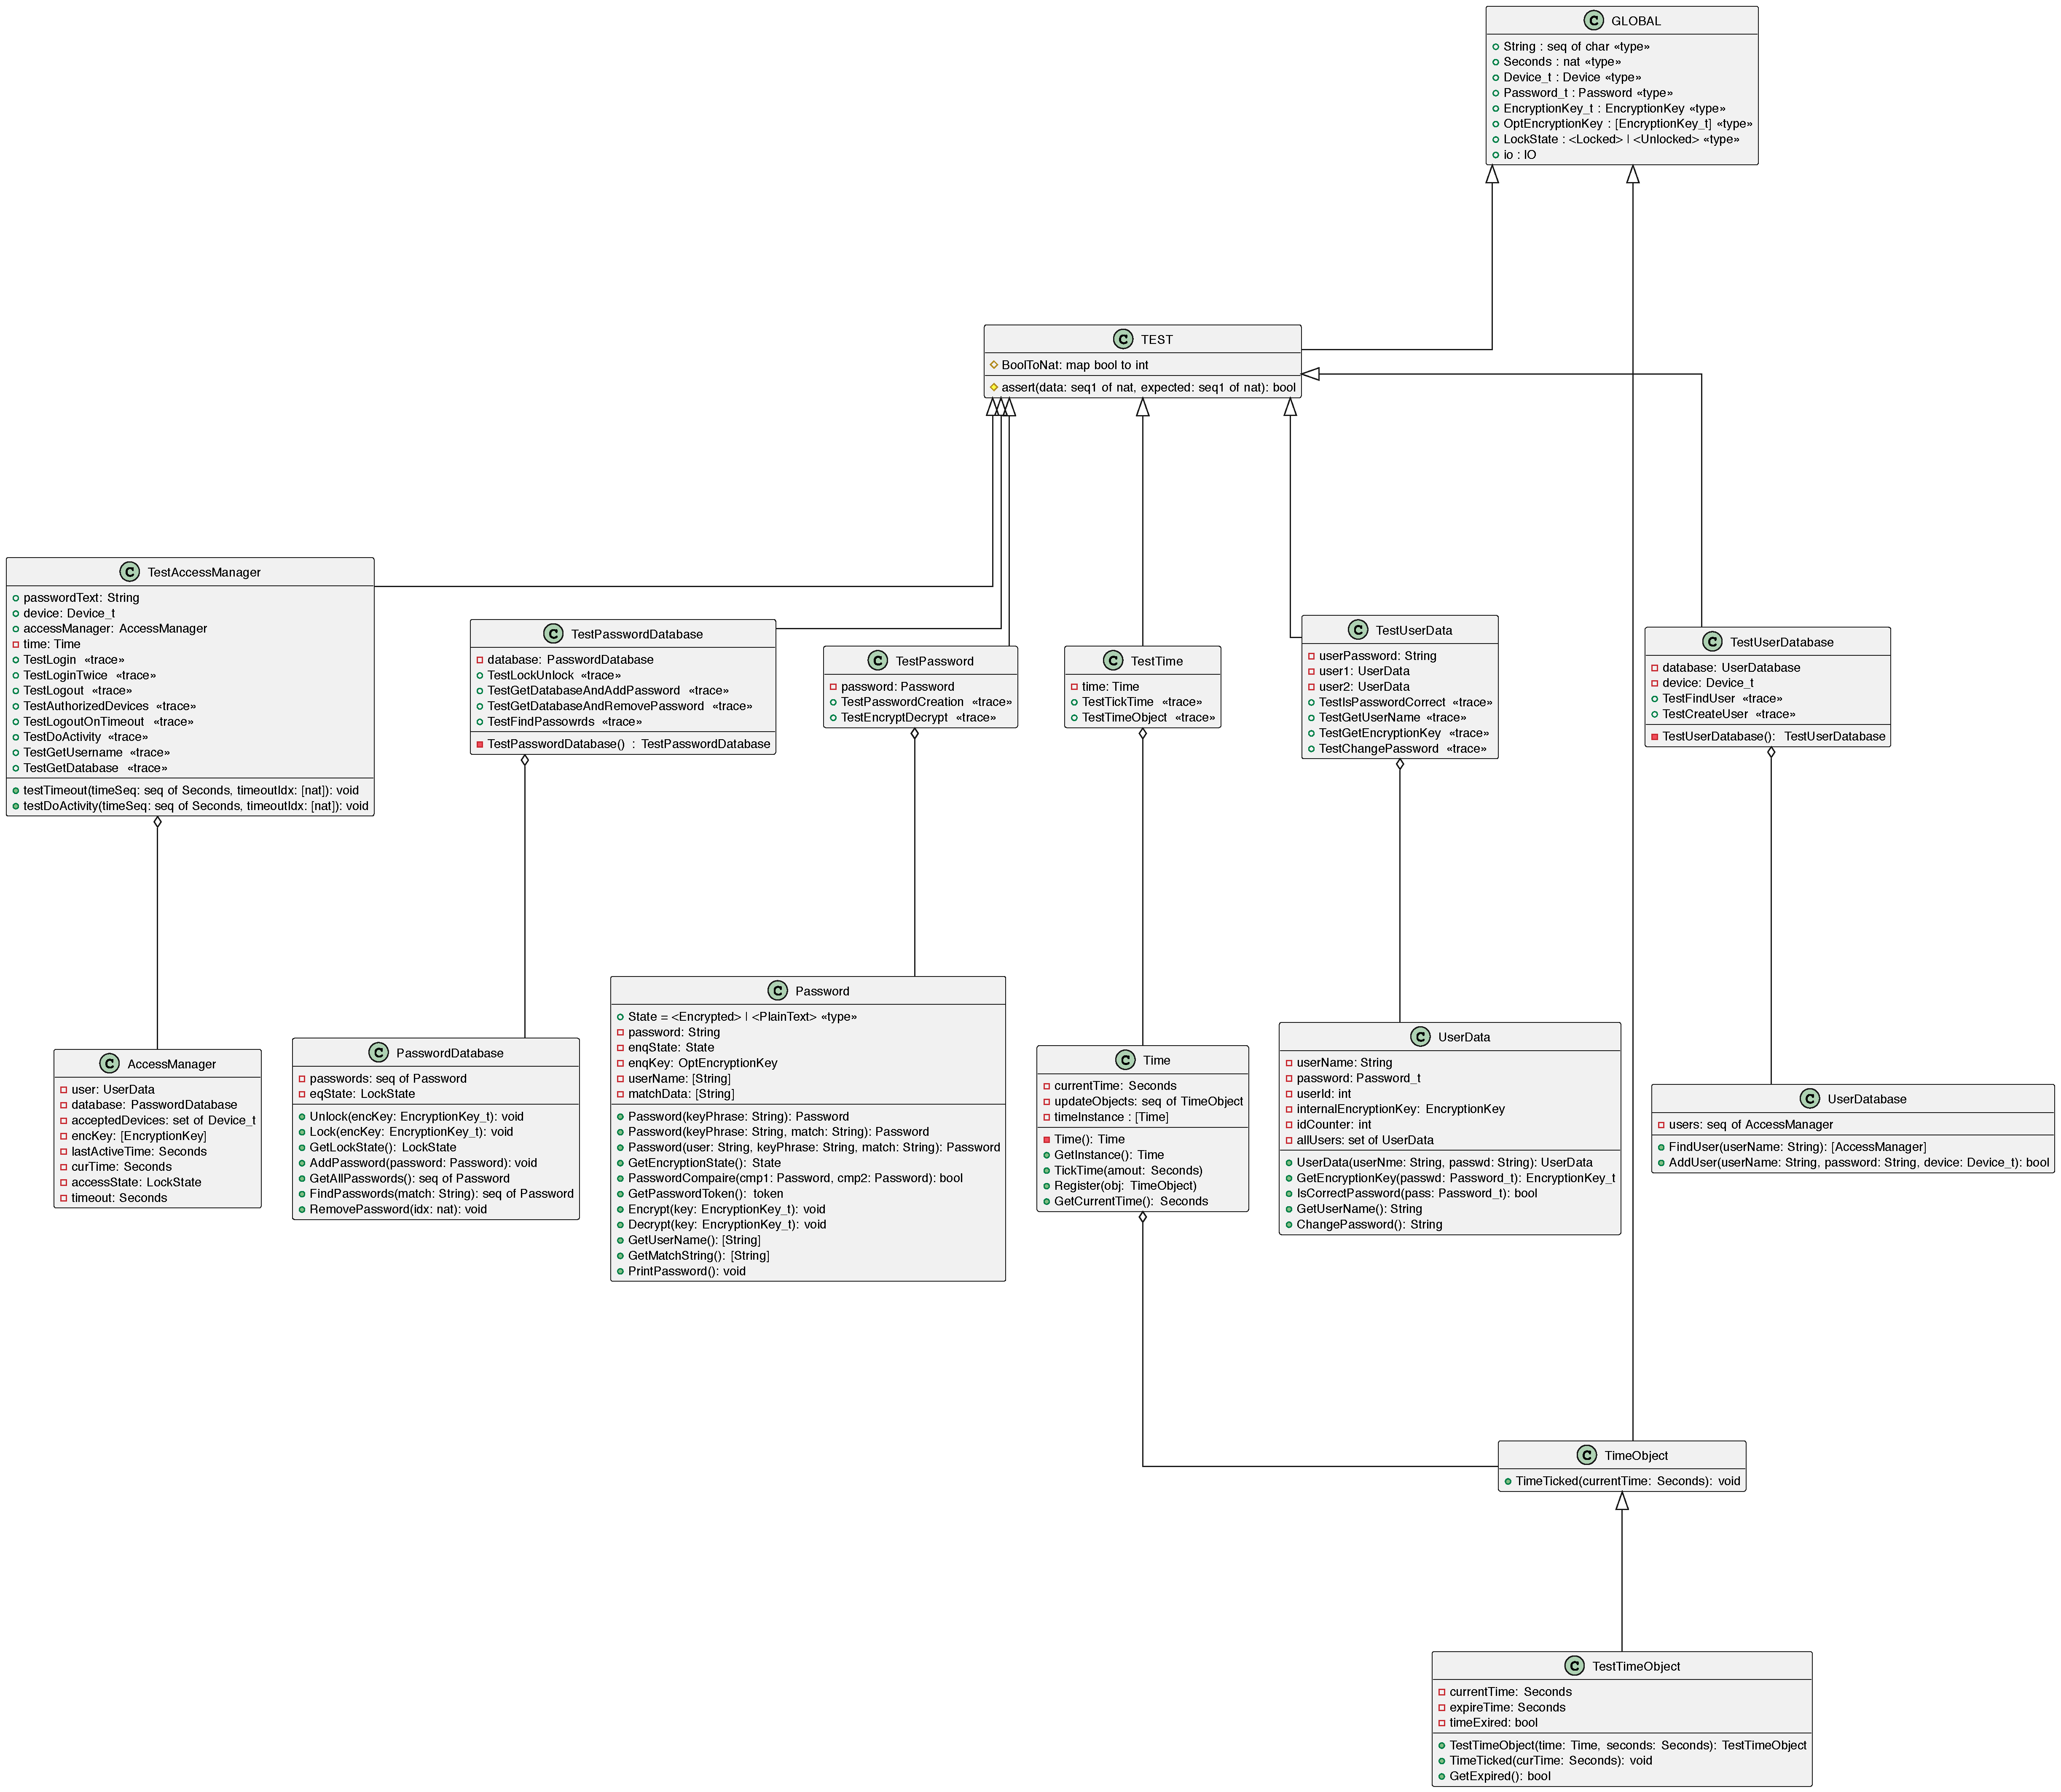
\includegraphics[width=13cm]{prj/figs/Test.pdf}
    \caption{Class diagram for the unit testing the password manager.}
    \label{fig:design:test}
\end{figure}

Here traces for each class is made to make sure that they preform as they
should. 

In the rest of this chapter functionalities of each class is highlighted.

\section{GLOBAL}
The global class is inherited by almost all other classes to provide basic
types to them. This includes the string type, but it also adds types of other
classes but where there equals operator is changed to compare members instead
of checking if the whole instance of the class is the same. How the global
class is implemented can be seen in \cref{lst:design:global}.
\begin{listing}[H]
    \begin{vdm_al}
class GLOBAL
types
public String = seq of char;

public Seconds = nat;

public Device_t = Device eq a = b == a.GetToken() = b.GetToken();

public Password_t = Password eq a = b == Password`PasswordCompaire(a,b);

public EncryptionKey_t = EncryptionKey eq a = b == a.GetToken() = b.GetToken();

public OptEncryptionKey = [EncryptionKey_t] eq a = b == if a = nil or b = nil
then a = nil and b = nil else (a.GetToken() = b.GetToken());

public LockState = <Locked> | <Unlocked>; instance variables public static io:
IO := new IO();

end GLOBAL

    \end{vdm_al}
    \caption{The GLOBAL class.}
    \label{lst:design:global}
\end{listing}

\section{World}
The world class is very simple what it does is initializing the environment and running it. The world class can be seen in \cref{lst:design:world}.

\begin{listing}[H]
    \begin{vdm_al}
class World
instance variables
    public static env: [Environment]:= nil;
operations
    public World :()==>World
    World() ==
    env := new Environment("scenario.txt");

    public Run :()==>()
    Run() ==
    (env.Run(););
end World
    

    \end{vdm_al}
    \caption{The world class.}
    \label{lst:design:world}
\end{listing}

\section{Environment}

The environment is a little more involved since it is wanted to do different actions while running  the scenario. Therefore there is made multiple helper functions that handles each given action for the scenario. To simplify how the actions types are specified each action have been given their ovn argument types even though some of the actions accepts the same argument types. The environment starts by creating the initial users in it's constructor and then running each action one by one. If some seconds are specified then it will also advance time to with the given Seconds. If no action is specified but a time interval is specified then it will just advance time without doing other actions. This creates a rather flexible environment class. How it runs the actions is shown in \cref{lst:design:env_run} where each action has an helper function.
\begin{listing}[H]
    \begin{vdm_al}
 public Run :()==>()
        Run() == 
            while len actions > 0 do
                (dcl
                    -- Preamble --
                    action : ActionsToDo := hd actions;
                    def mk_(timeTick, actionType, args) = action in(
                    io.print("\n-----------------\n");
                    -- Handle action --
                    if timeTick <> nil and timeTick <> 0 then
                        (time.TickTime(timeTick);
                        io.print("Time passed: ");
                        if(timeTick > 60) then
                            (io.print(timeTick div 60);io.print(" minutes "));
                        if((timeTick mod 60) <> 0) then
                            (io.print(timeTick mod 60);io.print(" seconds"));
                            io.print("\n"););
                        
                    cases actionType:
                    <Login> -> HandleLogin(args),
                    <Logout> -> HandleLogout(args),
                    <FindPass> -> HandleFindPass(args),
                    <AddPass> -> HandleAddPass(args),
                    <RMPass> -> HandleRMPass(args),
                    <AuthDevice> -> HandleAuthDevice(args),
                    <NewDevice> -> HandleNewDevice(args),
                    <FindUser> -> HandleFindUser(args)
                    end;
                    -- Postamble --
                    actions := tl actions;
                    io.print("-----------------\n");
                ));
    

    \end{vdm_al}
    \caption{The environment run function.}
    \label{lst:design:env_run}
\end{listing}

\section{Time}
Instead of just havening an abstract idea of what time is, and not having a specific interval for each time tick in this implantation the time class uses seconds to keep track of time. This is because the requirements specifies a specific time interval of 5 minutes for when the user should be logged out, and therefore it makes sense to use seconds and not just a abstract time counter when modeling the time in this system. Each time the time is advanced the time object also calls all registered {\ttfamily TimeObject}'s {\ttfamily TimeTicked} functions. How the time advances in the time class is done with the {\ttfamily TickTime} function and it is shown in \cref{lst:design:TickTime}. Due to time being global the time class is implemented as a singleton where you can get the global time instance with a static function.

\begin{listing}[H]
    \begin{vdm_al}
public TickTime: Seconds ==> ()
        TickTime(amout) == (currentTime := currentTime + amout;
            for all i in set inds updateObjects do
                updateObjects(i).TimeTicked(currentTime);
        );
    

    \end{vdm_al}
    \caption{The {\ttfamily TickTime} function.}
    \label{lst:design:TickTime}
\end{listing}
\section{TimeObject}
The time object class is an abstract helper class that allows for the time class for informing it when time advances. Though multiple classes would be able to inherit and implement this class since only the {\ttfamily AccessManager} needs to be able to keep track of time, it is the only class inheriting from this class in this model. The implementation of this class is very simple at it is each subclass' responsibility to implement the {\ttfamily TimeTicked} function. The implantation of the {\ttfamily TimeObject} is shown in \cref{lst:design:TimeObject}.

\begin{listing}[H]
    \begin{vdm_al}
class TimeObject is subclass of GLOBAL
operations
    public TimeTicked: Seconds ==> ()
    TimeTicked(currentTime) == 
        is not yet specified
end TimeObject

    \end{vdm_al}
    \caption{The {\ttfamily TimeObject} class.}
    \label{lst:design:TimeObject}
\end{listing}
\section{UserDatabase}
The user database holds a list of all Users. Since Each user is having a {\ttfamily AccessManager} the list of all users is a sequence of {\ttfamily AccessManager}'s. Due to the {\ttfamily UserData} constructor having a preamble that requires each username to be unique, the user database makes sure that when you add a user the user name is not already used as shown in \cref{lst:design:AddUser}.
\begin{listing}[H]
    \begin{vdm_al}
public AddUser: String * String * Device_t ==> bool
    AddUser(userName, password, device) ==
        (for all i in set inds users do
            if users(i).GetUserName() = userName then
                (io.print("Could not add user, username already exits!\n"); 
                 return false);
        users := users ^ [new AccessManager(userName, password, device)];
        return true);

    \end{vdm_al}
    \caption{The {\ttfamily AddUser} function.}
    \label{lst:design:AddUser}
\end{listing}
\section{AccessManager}
The access manager has the responsibility to manage login and logout of each user, where only approved devices should be able to login. When the correct password is given from a approved device the database for that given user is decrypted and the user can access their passwords. The access manager also logs out of the user when the user has been inactive for 5 minutes with the function shown in \cref{lst:design:TimeTicked}.

\begin{listing}[H]
    \begin{vdm_al}
    public TimeTicked: Seconds ==> ()
    TimeTicked(currentTime) == (
        if encKey <> nil and lastActiveTime + timeout <= currentTime then
            (dcl foo: bool; foo := Logout();
             io.print("User: ");
             io.print(GetUserName());
             io.print(", Logged out! User was inactive for too long.\n"));
        curTime := currentTime
    )
    \end{vdm_al}
    \caption{The {\ttfamily TimeTicked} function.}
    \label{lst:design:TimeTicked}
\end{listing}
\section{UserData}
The {\ttfamily UserData} class is responsible for holding the user information like user name and password, but also to generate the unique encryption key for the given user. How the encryption key is generated is show in \cref{lst:design:GetEncryptionKey} and is only how it is generated in the model and not representable as a real way to generate secure encryption keys.

\begin{listing}[H]
    \begin{vdm_al}
    public GetEncryptionKey: Password_t ==> EncryptionKey_t
        GetEncryptionKey(passwd) ==
        return new EncryptionKey(userId, passwd)
        pre password = passwd;
    \end{vdm_al}
    \caption{The {\ttfamily GetEncryptionKey} function.}
    \label{lst:design:GetEncryptionKey}
\end{listing}
\section{Password}
Passwords is holding their password and can hold a match string and a username. It has two overloaded constructors that allows it to be created with just the data needed as shown in \cref{lst:design:Password}


\begin{listing}[H]
    \begin{vdm_al}
       public Password: String ==> Password
    Password(keyPhrase) ==
        (password := keyPhrase;
         enqState := <PlainText>;
         enqKey := nil;
        );

    public Password: String * String ==> Password
    Password(keyPhrase, match) ==
        (password := keyPhrase;
         enqState := <PlainText>;
         enqKey := nil;
         matchData := match;
        );

    public Password: String * String * String ==> Password
    Password(user, keyPhrase, match) ==
        (password := keyPhrase;
         enqState := <PlainText>;
         enqKey := nil;
         matchData := match;
         userName := user;
        );
    \end{vdm_al}
    \caption{The {\ttfamily GetEncryptionKey} function.}
    \label{lst:design:Password}
\end{listing}
\section{PasswordDatabase}
The password database holds a users passwords. Do to it using the match string of the password to locate the given password in the database the password database has a invariant that all passwords needs to have a match string as shown in \cref{lst:design:PasswordDatabaseInv}.
\begin{listing}[H]
    \begin{vdm_al}
inv forall password in seq passwords & password.GetMatchString() <> nil;
    \end{vdm_al}
    \caption{The {\ttfamily PasswordDatabase} invariant.}
    \label{lst:design:PasswordDatabaseInv}
\end{listing}
\section{Device and EncryptionKey}
Both the Device class and EncryptionKey are very simple, and could probably be modeled just as named types, but to make it clear how to create these objects correctly, they are made into classes with specific constructors. This has the drawback that special equality operators needs to be implemented to compare them correctly, however it ensures that the device and encryption keys are generated correct with constructors that facilitates this. The constructor of EncryptionKey can be seen in \cref{lst:design:EncryptionKey}.
\begin{listing}[H]
    \begin{vdm_al}
public EncryptionKey: int * Password ==> EncryptionKey
    EncryptionKey(keyId, passwd) ==
        (keyToken := mk_token({keyId, passwd.GetPasswordToken()}));
    \end{vdm_al}
    \caption{The {\ttfamily PasswordDatabase} invariant.}
    \label{lst:design:EncryptionKey}
\end{listing}
